\chapter{Background \& Objectives}

This section should discuss your preparation for the project, including background reading, your analysis of the problem and the process or method you have followed to help structure your work.  It is likely that you will reuse part of your outline project specification, but at this point in the project you should have more to talk about. 

\textbf{Note}: 

\begin{itemize}
   \item All of the sections and text in this example are for illustration purposes. The main Chapters are a good starting point, but the content and actual sections that you include are likely to be different.
   
   \item Look at the document on the Structure of the Final Report for additional guidance. 
   
\end {itemize}

\subsection{SLAM - Simultaneous Localization And Mapping}
The SLAM problem is a current research topic which is based on different localisation algorithms and using a range of different sensor to effectively map an target area. A lot of different approaches have been done and many research papers have been written, the one this project is based on is a paper about a SLAM solution designed for autonomous vehicles\cite{Dissanayake2001Solution}.\\
While the research area of this paper is based on a much larger scale, it does still give me an insight upon the SLAM problem.\\
E.g. the problem with localisation in an dynamic environment, the paper tackles this problem by using global reference points and a millimetre wave radar, however for my project I do use an static environment and simple laser range finders. So this paper is only used a reference to the localisation problem, especially the idea of using "global" reference points for the created map.\\
As the test environment and the sensors available for the E-puck sensors are limited this project will assume that the starting location of the robots is known.\\[3ex]

Another paper which was read about this problem used an approach much more similar to this project, by using different mobile robots which have no GPS access and simply use 2D laser range finders. However the approach described in this paper was based around the mapping of one "lead" robot and the traversing the same map again with a second robot using the map generated by the first for localisation purposes.\\
The second robot would then scan the target area again and refine the already generated map though using the (now stationary) first robot as an reference point. Since this project is using single a robot for mapping purposes and multi robot usage would only be added if enough time is available, this paper was not inherently useful, however gave some useful insight for information sharing between robots or sensor stations as well as localisation of robots using a global reference point.\\
Since this project aims at real time localisation and mapping communication with a "uplink" point would be essential to achieve this in a real world setting. By using a similar implementation to the one described in the paper it would be possible to rescan a mapped area if it is traversed again, and by that refine the mapping. This is requires however very good localisation techniques.

\subsection{Deployment}
The deployment strategy is an important part of this project as it defines how effective the robot will cover the target area which will define how long it will take to scan and map the whole area. 
One research paper which was read proposed an solution of a communication network where the comm nodes keep track of the robots positions and guide them in directions which have not been explored in the last time period\cite{Batalin2003Coverage}. The paper uses a solution which is based on small comm nodes deployed by the robot, to make the solution fitting for this project the developer would have to use multiple E-Pucks and define some of these as communication nodes which remain on a fast position and guide the "scout" E-puck based on area which have been least visited by the other robots.\\ 
However since multi-robot usage is planned as an addition if enough time is available this deployment strategy is not fitting for the major part of work.

This would therefore need both a lead robot which decides the movement of the swarm and communication robots which would always have at least 1 link to another comm robot in order to have a communication line back to the lead robot. \\
This is one of two 2 deployment strategies I will try to implement during the testing period and try to find out which one would be more fitting for my project.\\[3ex]



\subsection{Communication}
While it is possible for me to transfer information easily between robots since I am using a simulator I am still trying implement it as close to a realistic scenario as possible, meaning that the communication range for the robots is limited. In an realistic scenario every robot would have to send the acquired map back to the static start point/lead robot so that an overall map of the environment can be created. \\
Since the communication range for such small robots is limited and can be even further obstructed through obstacles like walls it is important to designated some robots as communication nodes. Such comm nodes would than remain stationary and link the "scout" robots, which do the exploration, back to do the lead robot. \\
Obviously the most effective way to do this is by implementing different behaviour patterns for scouts or comm robots, and implement a decision model which allows the robot to change between either pattern as the needs of the swarm change. E.g. in the start of the exploration no comm robots will be needed as the robots would most likely be inside the comm range of the lead robot, though this may change if the swarm is big and spread out enough. \\[3ex]

To surpass the problems of obstacles obstructing the communication the comm robots would need to position them self on logical places i.e. in order to scan a room it would be important that a comm robot places it self inside, or close to, the doorway so that others can explore the room and still communicated back to the rest of the swarm. The robot would need to stay inside the doorway as signals can not always travel through walls and the energy reserves of mobile robots are limited so they most likely can not send high power signals. \\
I have yet to decide how I am going to implement the communication part of in the project as I am not sure if the E-puck models implemented inside the simulator are able to send signals to other robots. While I know that it is able to transfer signals through the E-puck's laser sensors I do not know if I will implement it as this is fairly difficult and time consuming. I will come back to this should I have enough time available at the end of the project or if no other alternative can be found.\\[3ex]

The theory of what I am going to implement uses a defined maximum communication range for the robots and a grouping strategy which specifies that each scout robot need to stay in contact which at least 1 comm robot while the comm robots always need at least 1 other comm robot inside their communication range. If implemented correctly the comm robots would on this way create a communication link back to the lead robot/starting location which the scout robots can use to transfer all new information back.\\

\begin{figure}[h]
\centering
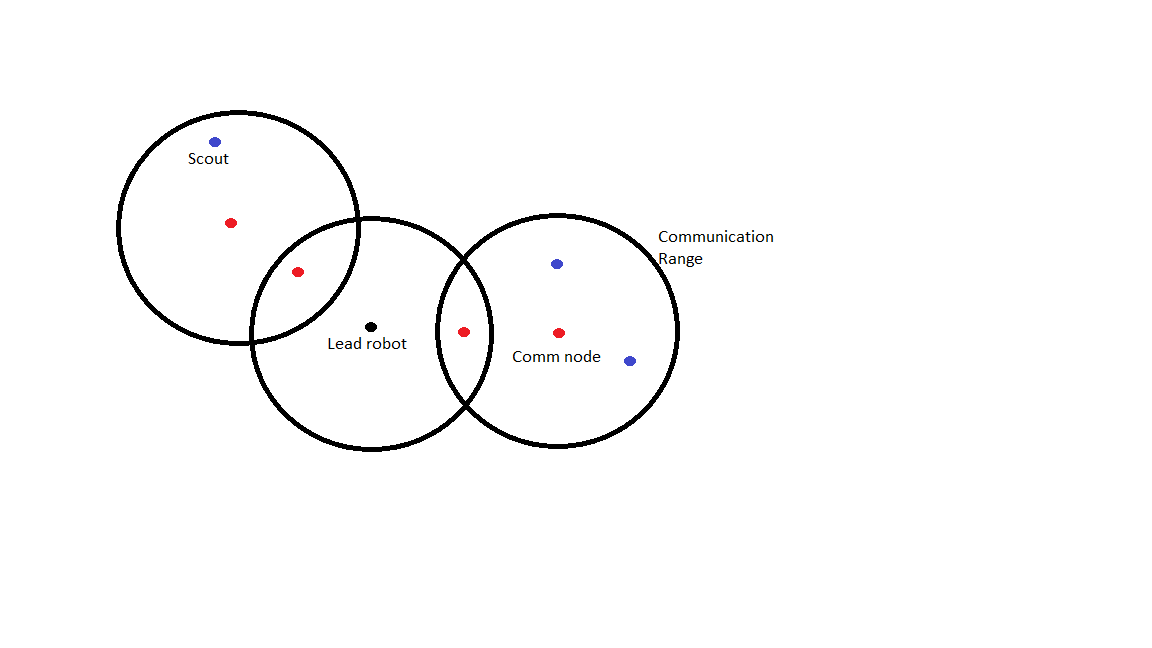
\includegraphics[width = 0.8\textwidth]{../../figures/comm_example.png} 
\caption{An example of the communication link}
\label{Figure 1}
\end{figure}

Figure 1 shows one possible example of the communication link, where the lead robot/ or in some cases a stationary uplink point is in the center and the communication robots(in red) placed in such positions that their comm range overlaps the comm range of other robots and the lead robot. \\
This configuration allows the scouts(in blue) to move and explore anything inside the communication range of the different comm robots. When the robots at the right side of the figure would now try to move outside the comm range one of them would have to change their behaviour pattern to "communication mode" at the outer range of the other comm nodes range while the last remaining scout continuous exploring in this direction. \\
This example shows that it is important to have a swarm of a suitable size for an environment to be able to cover at much area with the robots at hand and for cases in which this is not possible to be able to move the whole swarm in one unified direction to explore unmapped locations. This is however only doable when there is a lead robot since a stationary comm/uplink point is by definition, stationary.\\

\section{Analysis}
Taking into account the problem and what you learned from the background work, what was your analysis of the problem? How did your analysis help to decompose the problem into the main tasks that you would undertake? Were there alternative approaches? Why did you choose one approach compared to the alternatives? 

There should be a clear statement of the objectives of the work, which you will evaluate at the end of the work. 

In most cases, the agreed objectives or requirements will be the result of a compromise between what would ideally have been produced and what was felt to be possible in the time available. A discussion of the process of arriving at the final list is usually appropriate.

\section{Process}
You need to describe briefly the life cycle model or research method that you used. You do not need to write about all of the different process models that you are aware of. Focus on the process model that you have used. It is possible that you needed to adapt an existing process model to suit your project; clearly identify what you used and how you adapted it for your needs.

